% Options for packages loaded elsewhere
\PassOptionsToPackage{unicode}{hyperref}
\PassOptionsToPackage{hyphens}{url}
%
\documentclass[
]{article}
\usepackage{lmodern}
\usepackage{amsmath}
\usepackage{ifxetex,ifluatex}
\ifnum 0\ifxetex 1\fi\ifluatex 1\fi=0 % if pdftex
  \usepackage[T1]{fontenc}
  \usepackage[utf8]{inputenc}
  \usepackage{textcomp} % provide euro and other symbols
  \usepackage{amssymb}
\else % if luatex or xetex
  \usepackage{unicode-math}
  \defaultfontfeatures{Scale=MatchLowercase}
  \defaultfontfeatures[\rmfamily]{Ligatures=TeX,Scale=1}
\fi
% Use upquote if available, for straight quotes in verbatim environments
\IfFileExists{upquote.sty}{\usepackage{upquote}}{}
\IfFileExists{microtype.sty}{% use microtype if available
  \usepackage[]{microtype}
  \UseMicrotypeSet[protrusion]{basicmath} % disable protrusion for tt fonts
}{}
\makeatletter
\@ifundefined{KOMAClassName}{% if non-KOMA class
  \IfFileExists{parskip.sty}{%
    \usepackage{parskip}
  }{% else
    \setlength{\parindent}{0pt}
    \setlength{\parskip}{6pt plus 2pt minus 1pt}}
}{% if KOMA class
  \KOMAoptions{parskip=half}}
\makeatother
\usepackage{xcolor}
\IfFileExists{xurl.sty}{\usepackage{xurl}}{} % add URL line breaks if available
\IfFileExists{bookmark.sty}{\usepackage{bookmark}}{\usepackage{hyperref}}
\hypersetup{
  pdftitle={Assignment 1 -- Experimental Design and Data Analysis},
  hidelinks,
  pdfcreator={LaTeX via pandoc}}
\urlstyle{same} % disable monospaced font for URLs
\usepackage[margin=1in]{geometry}
\usepackage{color}
\usepackage{fancyvrb}
\newcommand{\VerbBar}{|}
\newcommand{\VERB}{\Verb[commandchars=\\\{\}]}
\DefineVerbatimEnvironment{Highlighting}{Verbatim}{commandchars=\\\{\}}
% Add ',fontsize=\small' for more characters per line
\usepackage{framed}
\definecolor{shadecolor}{RGB}{248,248,248}
\newenvironment{Shaded}{\begin{snugshade}}{\end{snugshade}}
\newcommand{\AlertTok}[1]{\textcolor[rgb]{0.94,0.16,0.16}{#1}}
\newcommand{\AnnotationTok}[1]{\textcolor[rgb]{0.56,0.35,0.01}{\textbf{\textit{#1}}}}
\newcommand{\AttributeTok}[1]{\textcolor[rgb]{0.77,0.63,0.00}{#1}}
\newcommand{\BaseNTok}[1]{\textcolor[rgb]{0.00,0.00,0.81}{#1}}
\newcommand{\BuiltInTok}[1]{#1}
\newcommand{\CharTok}[1]{\textcolor[rgb]{0.31,0.60,0.02}{#1}}
\newcommand{\CommentTok}[1]{\textcolor[rgb]{0.56,0.35,0.01}{\textit{#1}}}
\newcommand{\CommentVarTok}[1]{\textcolor[rgb]{0.56,0.35,0.01}{\textbf{\textit{#1}}}}
\newcommand{\ConstantTok}[1]{\textcolor[rgb]{0.00,0.00,0.00}{#1}}
\newcommand{\ControlFlowTok}[1]{\textcolor[rgb]{0.13,0.29,0.53}{\textbf{#1}}}
\newcommand{\DataTypeTok}[1]{\textcolor[rgb]{0.13,0.29,0.53}{#1}}
\newcommand{\DecValTok}[1]{\textcolor[rgb]{0.00,0.00,0.81}{#1}}
\newcommand{\DocumentationTok}[1]{\textcolor[rgb]{0.56,0.35,0.01}{\textbf{\textit{#1}}}}
\newcommand{\ErrorTok}[1]{\textcolor[rgb]{0.64,0.00,0.00}{\textbf{#1}}}
\newcommand{\ExtensionTok}[1]{#1}
\newcommand{\FloatTok}[1]{\textcolor[rgb]{0.00,0.00,0.81}{#1}}
\newcommand{\FunctionTok}[1]{\textcolor[rgb]{0.00,0.00,0.00}{#1}}
\newcommand{\ImportTok}[1]{#1}
\newcommand{\InformationTok}[1]{\textcolor[rgb]{0.56,0.35,0.01}{\textbf{\textit{#1}}}}
\newcommand{\KeywordTok}[1]{\textcolor[rgb]{0.13,0.29,0.53}{\textbf{#1}}}
\newcommand{\NormalTok}[1]{#1}
\newcommand{\OperatorTok}[1]{\textcolor[rgb]{0.81,0.36,0.00}{\textbf{#1}}}
\newcommand{\OtherTok}[1]{\textcolor[rgb]{0.56,0.35,0.01}{#1}}
\newcommand{\PreprocessorTok}[1]{\textcolor[rgb]{0.56,0.35,0.01}{\textit{#1}}}
\newcommand{\RegionMarkerTok}[1]{#1}
\newcommand{\SpecialCharTok}[1]{\textcolor[rgb]{0.00,0.00,0.00}{#1}}
\newcommand{\SpecialStringTok}[1]{\textcolor[rgb]{0.31,0.60,0.02}{#1}}
\newcommand{\StringTok}[1]{\textcolor[rgb]{0.31,0.60,0.02}{#1}}
\newcommand{\VariableTok}[1]{\textcolor[rgb]{0.00,0.00,0.00}{#1}}
\newcommand{\VerbatimStringTok}[1]{\textcolor[rgb]{0.31,0.60,0.02}{#1}}
\newcommand{\WarningTok}[1]{\textcolor[rgb]{0.56,0.35,0.01}{\textbf{\textit{#1}}}}
\usepackage{graphicx}
\makeatletter
\def\maxwidth{\ifdim\Gin@nat@width>\linewidth\linewidth\else\Gin@nat@width\fi}
\def\maxheight{\ifdim\Gin@nat@height>\textheight\textheight\else\Gin@nat@height\fi}
\makeatother
% Scale images if necessary, so that they will not overflow the page
% margins by default, and it is still possible to overwrite the defaults
% using explicit options in \includegraphics[width, height, ...]{}
\setkeys{Gin}{width=\maxwidth,height=\maxheight,keepaspectratio}
% Set default figure placement to htbp
\makeatletter
\def\fps@figure{htbp}
\makeatother
\setlength{\emergencystretch}{3em} % prevent overfull lines
\providecommand{\tightlist}{%
  \setlength{\itemsep}{0pt}\setlength{\parskip}{0pt}}
\setcounter{secnumdepth}{-\maxdimen} % remove section numbering
\ifluatex
  \usepackage{selnolig}  % disable illegal ligatures
\fi

\title{Assignment 1 -- Experimental Design and Data Analysis}
\author{}
\date{\vspace{-2.5em}}

\begin{document}
\maketitle


\pagenumbering{gobble}

%\begin{titlepage}
\begin{center}
\LARGE{\textbf{Assignment 1}}\\
\normalsize{Experimental Design and Data Analysis}\\
\vspace*{2\baselineskip}

\vspace*{2\baselineskip}
\Large{Ramon Bussing}\\
\Large{Daan Moll}\\
\Large{Karim Semin}\\
\vspace*{3\baselineskip}

\vspace*{2\baselineskip}

\today
\end{center}
% \end{titlepage}

\doublespacing

\hypersetup{linkcolor = black}
\newpage
\pagenumbering{roman}
\newpage

\hypertarget{exercise-1}{%
\subsection{Exercise 1}\label{exercise-1}}

The data set birthweight.txt contains the birthweights of 188 newborn
babies. We are interested in finding the underlying (population) mean μ
of birthweights.

\begin{enumerate}
\def\labelenumi{\alph{enumi})}
\tightlist
\item
  Check normality of the data. Compute a point estimate for μ. Derive,
  assuming normality (irrespective of your conclusion about normality od
  the data), a bounded 90\% confidence interval for μ.
\end{enumerate}

Point estimate for μ:

\begin{Shaded}
\begin{Highlighting}[]
\FunctionTok{mean}\NormalTok{(birthweight)}
\end{Highlighting}
\end{Shaded}

\begin{verbatim}
## [1] 2913.293
\end{verbatim}

Check normality with Shapiro-Wilk test:

\begin{Shaded}
\begin{Highlighting}[]
\FunctionTok{shapiro.test}\NormalTok{(birthweight)[}\DecValTok{2}\NormalTok{]}
\end{Highlighting}
\end{Shaded}

\begin{verbatim}
## $p.value
## [1] 0.8995395
\end{verbatim}

p is non-significant. This implies that h0 is accepted (the data is
normally distributed).

\begin{enumerate}
\def\labelenumi{\alph{enumi})}
\setcounter{enumi}{1}
\tightlist
\item
  An expert claims that the mean birthweight is bigger than 2800, verify
  this claim by using a t-test. What is the outcome of the test if you
  take α = 0.1? And other values of α?
\end{enumerate}

If we test this hypothesis with α = 0.1 we get:

\begin{Shaded}
\begin{Highlighting}[]
\NormalTok{alpha }\OtherTok{=}\NormalTok{ .}\DecValTok{1}
\FunctionTok{t.test}\NormalTok{(birthweight, }\AttributeTok{alternative =} \StringTok{"l"}\NormalTok{, }\AttributeTok{conf.level =} \DecValTok{1}\SpecialCharTok{{-}}\NormalTok{alpha, }\AttributeTok{mu =} \DecValTok{2800}\NormalTok{)[}\DecValTok{3}\NormalTok{]}
\end{Highlighting}
\end{Shaded}

\begin{verbatim}
## $p.value
## [1] 0.9864326
\end{verbatim}

p = .9864, therefore, h0 is accepted. If we try this for alpha = .05,
.01, .001, we get the following p values:

\begin{Shaded}
\begin{Highlighting}[]
\NormalTok{alpha }\OtherTok{=}\NormalTok{ .}\DecValTok{05}
\FunctionTok{t.test}\NormalTok{(birthweight, }\AttributeTok{alternative =} \StringTok{"l"}\NormalTok{, }\AttributeTok{conf.level =} \DecValTok{1}\SpecialCharTok{{-}}\NormalTok{alpha, }\AttributeTok{mu =} \DecValTok{2800}\NormalTok{)[}\DecValTok{3}\NormalTok{]}
\end{Highlighting}
\end{Shaded}

\begin{verbatim}
## $p.value
## [1] 0.9864326
\end{verbatim}

\begin{Shaded}
\begin{Highlighting}[]
\NormalTok{alpha }\OtherTok{=}\NormalTok{ .}\DecValTok{05}
\end{Highlighting}
\end{Shaded}

\begin{enumerate}
\def\labelenumi{\alph{enumi})}
\setcounter{enumi}{2}
\tightlist
\item
  In the R-output of the test from b), also a confidence interval is
  given, but why is it different from the confidence interval found in
  a) and why is it one-sided?
\end{enumerate}

\hypertarget{exercise-2}{%
\subsection{Exercise 2}\label{exercise-2}}

We study the power function of the two-sample t-test (see Section 1.9 of
Assignment 0). For n=m=30, mu=180, nu=175 and sd=5, generate 1000
samples x=rnorm(n,mu,sd) and y=rnorm(m,nu,sd), and record the 1000
p-values for testing H0: mu=nu. You can evaluate the power (at point
nu=175) of this t-test as fraction of p-values that are smaller than
0.05.

\begin{Shaded}
\begin{Highlighting}[]
\NormalTok{n}\OtherTok{=}\NormalTok{m}\OtherTok{=}\DecValTok{30}
\NormalTok{mu}\OtherTok{=}\DecValTok{180}
\NormalTok{nu}\OtherTok{=}\DecValTok{175}
\NormalTok{sd}\OtherTok{=}\DecValTok{5}

\NormalTok{B}\OtherTok{=}\DecValTok{1000}
\NormalTok{p}\OtherTok{=}\FunctionTok{numeric}\NormalTok{(B)}
\ControlFlowTok{for}\NormalTok{ (b }\ControlFlowTok{in} \DecValTok{1}\SpecialCharTok{:}\NormalTok{B) \{}
\NormalTok{  x}\OtherTok{=}\FunctionTok{rnorm}\NormalTok{(n,mu,sd);}
\NormalTok{  y}\OtherTok{=}\FunctionTok{rnorm}\NormalTok{(m,nu,sd);}
\NormalTok{  p[b]}\OtherTok{=}\FunctionTok{t.test}\NormalTok{(x,y,}\AttributeTok{var.equal =} \ConstantTok{TRUE}\NormalTok{)[[}\DecValTok{3}\NormalTok{]]\}}
\NormalTok{a }\OtherTok{\textless{}{-}} \FunctionTok{table}\NormalTok{(p)}
\FunctionTok{length}\NormalTok{(a[}\FunctionTok{names}\NormalTok{(a)}\SpecialCharTok{\textless{}}\FloatTok{0.05}\NormalTok{])}\SpecialCharTok{/}\FunctionTok{length}\NormalTok{(a)}
\end{Highlighting}
\end{Shaded}

\begin{verbatim}
## [1] 0.59
\end{verbatim}

\begin{enumerate}
\def\labelenumi{\alph{enumi})}
\tightlist
\item
  Set n=m=30, mu=180 and sd=5. Calculate now the power of the t-test for
  every value of nu in the grid seq(175,185,by=0.25). Plot the power as
  a function of nu.
\end{enumerate}

\begin{Shaded}
\begin{Highlighting}[]
\NormalTok{n}\OtherTok{=}\NormalTok{m}\OtherTok{=}\DecValTok{30}
\NormalTok{mu}\OtherTok{=}\DecValTok{180}
\NormalTok{nus}\OtherTok{=}\FunctionTok{seq}\NormalTok{(}\DecValTok{175}\NormalTok{,}\DecValTok{185}\NormalTok{,}\AttributeTok{by=}\FloatTok{0.25}\NormalTok{)}
\NormalTok{sd}\OtherTok{=}\DecValTok{5}

\NormalTok{powers }\OtherTok{=} \FunctionTok{numeric}\NormalTok{(}\FunctionTok{length}\NormalTok{(nus))}

\NormalTok{B}\OtherTok{=}\DecValTok{1000}
\NormalTok{p}\OtherTok{=}\FunctionTok{numeric}\NormalTok{(B)}
\ControlFlowTok{for}\NormalTok{ (i }\ControlFlowTok{in} \DecValTok{1}\SpecialCharTok{:}\FunctionTok{length}\NormalTok{(nus)) \{}
\NormalTok{  nu }\OtherTok{=}\NormalTok{ nus[i]}
  \ControlFlowTok{for}\NormalTok{ (b }\ControlFlowTok{in} \DecValTok{1}\SpecialCharTok{:}\NormalTok{B) \{}
\NormalTok{    x}\OtherTok{=}\FunctionTok{rnorm}\NormalTok{(n,mu,sd);}
\NormalTok{    y}\OtherTok{=}\FunctionTok{rnorm}\NormalTok{(m,nu,sd);}
\NormalTok{    p[b]}\OtherTok{=}\FunctionTok{t.test}\NormalTok{(x,y,}\AttributeTok{var.equal =} \ConstantTok{TRUE}\NormalTok{)[[}\DecValTok{3}\NormalTok{]]\}}
\NormalTok{  a }\OtherTok{\textless{}{-}} \FunctionTok{table}\NormalTok{(p)}
\NormalTok{  powers[i] }\OtherTok{=} \FunctionTok{length}\NormalTok{(a[}\FunctionTok{names}\NormalTok{(a)}\SpecialCharTok{\textless{}}\FloatTok{0.05}\NormalTok{])}\SpecialCharTok{/}\FunctionTok{length}\NormalTok{(a)}
\NormalTok{\} }
\NormalTok{powers\_a }\OtherTok{=}\NormalTok{ powers}
\NormalTok{nus\_a }\OtherTok{=}\NormalTok{ nus}

\NormalTok{plot1 }\OtherTok{=} \FunctionTok{plot}\NormalTok{(nus\_a, powers\_a)}
\end{Highlighting}
\end{Shaded}

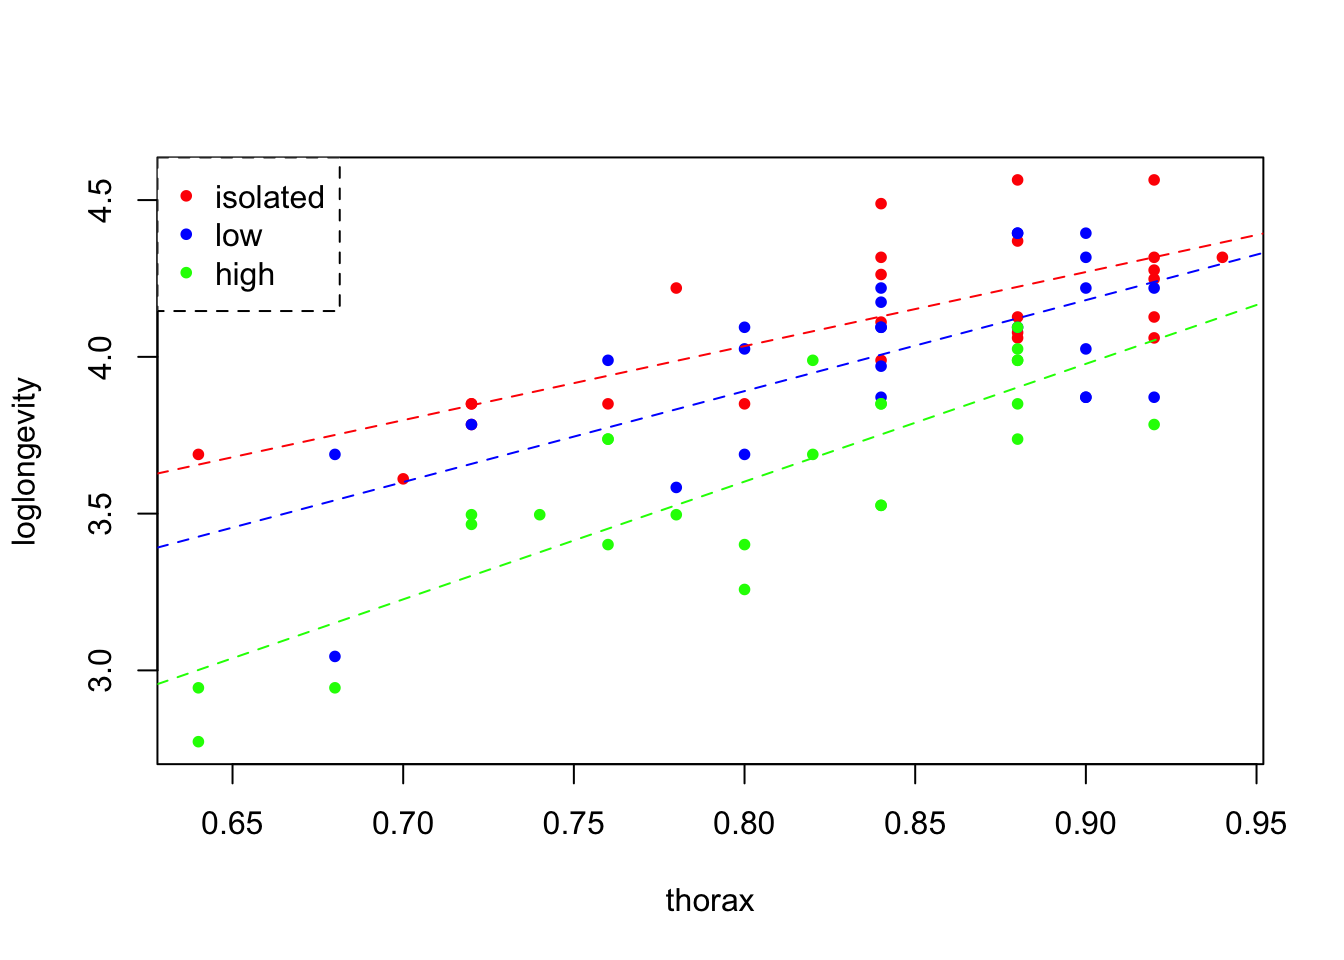
\includegraphics{assignment1_files/figure-latex/unnamed-chunk-7-1.pdf}

\begin{enumerate}
\def\labelenumi{\alph{enumi})}
\setcounter{enumi}{1}
\tightlist
\item
  Set n=m=100, mu=180 and sd=5. Repeat the preceding exercise. Add the
  plot to the preceding plot.
\end{enumerate}

\begin{Shaded}
\begin{Highlighting}[]
\NormalTok{n}\OtherTok{=}\NormalTok{m}\OtherTok{=}\DecValTok{100}
\NormalTok{mu}\OtherTok{=}\DecValTok{180}
\NormalTok{nus}\OtherTok{=}\FunctionTok{seq}\NormalTok{(}\DecValTok{175}\NormalTok{,}\DecValTok{185}\NormalTok{,}\AttributeTok{by=}\FloatTok{0.25}\NormalTok{)}
\NormalTok{sd}\OtherTok{=}\DecValTok{5}

\NormalTok{powers }\OtherTok{=} \FunctionTok{numeric}\NormalTok{(}\FunctionTok{length}\NormalTok{(nus))}

\NormalTok{B}\OtherTok{=}\DecValTok{1000}
\NormalTok{p}\OtherTok{=}\FunctionTok{numeric}\NormalTok{(B)}
\ControlFlowTok{for}\NormalTok{ (i }\ControlFlowTok{in} \DecValTok{1}\SpecialCharTok{:}\FunctionTok{length}\NormalTok{(nus)) \{}
\NormalTok{  nu }\OtherTok{=}\NormalTok{ nus[i]}
  \ControlFlowTok{for}\NormalTok{ (b }\ControlFlowTok{in} \DecValTok{1}\SpecialCharTok{:}\NormalTok{B) \{}
\NormalTok{    x}\OtherTok{=}\FunctionTok{rnorm}\NormalTok{(n,mu,sd);}
\NormalTok{    y}\OtherTok{=}\FunctionTok{rnorm}\NormalTok{(m,nu,sd);}
\NormalTok{    p[b]}\OtherTok{=}\FunctionTok{t.test}\NormalTok{(x,y,}\AttributeTok{var.equal =} \ConstantTok{TRUE}\NormalTok{)[[}\DecValTok{3}\NormalTok{]]\}}
\NormalTok{  a }\OtherTok{\textless{}{-}} \FunctionTok{table}\NormalTok{(p)}
\NormalTok{  powers[i] }\OtherTok{=} \FunctionTok{length}\NormalTok{(a[}\FunctionTok{names}\NormalTok{(a)}\SpecialCharTok{\textless{}}\FloatTok{0.05}\NormalTok{])}\SpecialCharTok{/}\FunctionTok{length}\NormalTok{(a)}
\NormalTok{\} }
\NormalTok{powers\_b }\OtherTok{=}\NormalTok{ powers}
\NormalTok{nus\_b }\OtherTok{=}\NormalTok{ nus}

\NormalTok{plot2 }\OtherTok{=} \FunctionTok{plot}\NormalTok{(nus, powers)}
\end{Highlighting}
\end{Shaded}

\includegraphics{assignment1_files/figure-latex/unnamed-chunk-8-1.pdf}

\begin{enumerate}
\def\labelenumi{\alph{enumi})}
\setcounter{enumi}{2}
\tightlist
\item
  Set n=m=30, mu=180 and sd=15. Repeat the preceding exercise.
\end{enumerate}

\begin{Shaded}
\begin{Highlighting}[]
\NormalTok{n}\OtherTok{=}\NormalTok{m}\OtherTok{=}\DecValTok{30}
\NormalTok{mu}\OtherTok{=}\DecValTok{180}
\NormalTok{nus}\OtherTok{=}\FunctionTok{seq}\NormalTok{(}\DecValTok{175}\NormalTok{,}\DecValTok{185}\NormalTok{,}\AttributeTok{by=}\FloatTok{0.25}\NormalTok{)}
\NormalTok{sd}\OtherTok{=}\DecValTok{15}

\NormalTok{powers }\OtherTok{=} \FunctionTok{numeric}\NormalTok{(}\FunctionTok{length}\NormalTok{(nus))}

\NormalTok{B}\OtherTok{=}\DecValTok{1000}
\NormalTok{p}\OtherTok{=}\FunctionTok{numeric}\NormalTok{(B)}
\ControlFlowTok{for}\NormalTok{ (i }\ControlFlowTok{in} \DecValTok{1}\SpecialCharTok{:}\FunctionTok{length}\NormalTok{(nus)) \{}
\NormalTok{  nu }\OtherTok{=}\NormalTok{ nus[i]}
  \ControlFlowTok{for}\NormalTok{ (b }\ControlFlowTok{in} \DecValTok{1}\SpecialCharTok{:}\NormalTok{B) \{}
\NormalTok{    x}\OtherTok{=}\FunctionTok{rnorm}\NormalTok{(n,mu,sd);}
\NormalTok{    y}\OtherTok{=}\FunctionTok{rnorm}\NormalTok{(m,nu,sd);}
\NormalTok{    p[b]}\OtherTok{=}\FunctionTok{t.test}\NormalTok{(x,y,}\AttributeTok{var.equal =} \ConstantTok{TRUE}\NormalTok{)[[}\DecValTok{3}\NormalTok{]]\}}
\NormalTok{  a }\OtherTok{\textless{}{-}} \FunctionTok{table}\NormalTok{(p)}
\NormalTok{  powers[i] }\OtherTok{=} \FunctionTok{length}\NormalTok{(a[}\FunctionTok{names}\NormalTok{(a)}\SpecialCharTok{\textless{}}\FloatTok{0.05}\NormalTok{])}\SpecialCharTok{/}\FunctionTok{length}\NormalTok{(a)}
\NormalTok{\} }
\NormalTok{powers\_c }\OtherTok{=}\NormalTok{ powers}
\NormalTok{nus\_c }\OtherTok{=}\NormalTok{ nus}
\end{Highlighting}
\end{Shaded}

\begin{Shaded}
\begin{Highlighting}[]
\FunctionTok{par}\NormalTok{(}\AttributeTok{mfrow=}\FunctionTok{c}\NormalTok{(}\DecValTok{2}\NormalTok{,}\DecValTok{2}\NormalTok{))}
\FunctionTok{plot}\NormalTok{(nus\_a, powers\_a, }\AttributeTok{main=}\StringTok{"2a"}\NormalTok{, }\AttributeTok{xlab=}\StringTok{"nu"}\NormalTok{, }\AttributeTok{ylab=}\StringTok{"power"}\NormalTok{)}
\FunctionTok{plot}\NormalTok{(nus\_b, powers\_b, }\AttributeTok{main=}\StringTok{"2b"}\NormalTok{, }\AttributeTok{xlab=}\StringTok{"nu"}\NormalTok{, }\AttributeTok{ylab=}\StringTok{"power"}\NormalTok{)}
\FunctionTok{plot}\NormalTok{(nus\_c, powers\_c, }\AttributeTok{main=}\StringTok{"2c"}\NormalTok{, }\AttributeTok{xlab=}\StringTok{"nu"}\NormalTok{, }\AttributeTok{ylab=}\StringTok{"power"}\NormalTok{)}
\end{Highlighting}
\end{Shaded}

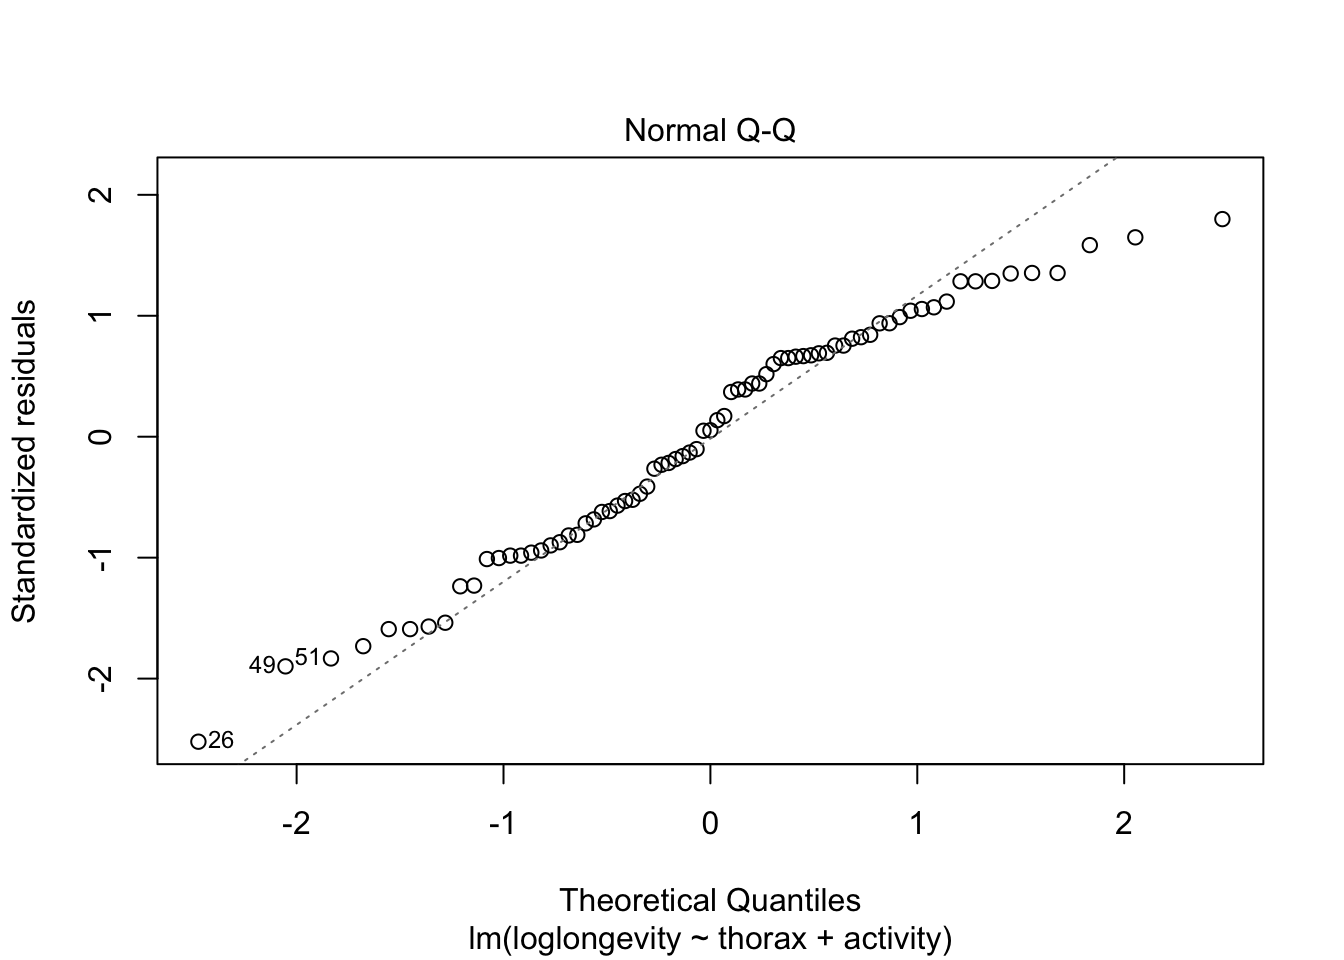
\includegraphics{assignment1_files/figure-latex/unnamed-chunk-9-1.pdf}

\begin{enumerate}
\def\labelenumi{\alph{enumi})}
\setcounter{enumi}{3}
\tightlist
\item
  Explain your findings.
\end{enumerate}

\hypertarget{exercise-3}{%
\subsection{Exercise 3}\label{exercise-3}}

A telecommunication company has entered the market for mobile phones in
a new country. The company's marketing manager conducts a survey of 200
new subscribers for mobile phones. The results of the survey are in the
data set telephone.txt, which contains the first month bills X1 , . . .
X200 , in euros.

\begin{enumerate}
\def\labelenumi{\alph{enumi})}
\tightlist
\item
  Make an appropriate plot of this data set. What marketing advice(s)
  would you give to the marketing manager? Are there any inconsistencies
  in the data? If so, try to fix these.
\end{enumerate}

\begin{Shaded}
\begin{Highlighting}[]
\NormalTok{telephone\_data }\OtherTok{=} \FunctionTok{read.table}\NormalTok{(}\StringTok{"telephone.txt"}\NormalTok{,}\AttributeTok{header=}\ConstantTok{TRUE}\NormalTok{)}

\CommentTok{\# sorted data of firsth month bills}
\FunctionTok{sort}\NormalTok{(telephone\_data}\SpecialCharTok{$}\NormalTok{Bills)}
\end{Highlighting}
\end{Shaded}

\begin{verbatim}
##   [1]   0.00   0.00   0.00   0.00   0.00   0.00   0.00   0.00   0.98   1.08
##  [11]   1.47   1.57   1.62   1.88   2.42   2.45   2.67   2.72   2.80   2.88
##  [21]   3.03   3.20   3.43   3.69   3.85   4.69   5.04   5.10   5.20   5.42
##  [31]   5.64   5.72   6.45   6.48   6.48   6.72   6.93   6.95   6.95   7.18
##  [41]   7.74   8.11   8.37   8.40   8.41   9.01   9.12   9.12   9.16   9.22
##  [51]   9.44   9.63  10.05  10.13  10.44  10.70  10.88  11.05  11.07  11.27
##  [61]  11.64  12.24  13.26  13.36  13.54  13.62  13.68  13.90  13.95  14.34
##  [71]  14.49  15.21  15.30  15.30  15.42  15.43  16.44  16.47  17.12  18.49
##  [81]  18.89  19.34  19.45  19.60  19.70  20.12  20.39  20.55  20.84  21.00
##  [91]  21.13  21.34  21.36  21.97  22.57  23.31  24.42  24.49  26.40  26.84
## [101]  26.97  27.21  27.57  28.77  29.04  29.23  29.24  29.25  30.61  30.62
## [111]  31.77  33.40  33.69  35.00  35.32  38.45  39.21  41.38  42.19  44.16
## [121]  44.32  45.77  45.81  48.54  49.24  53.21  53.90  55.99  56.01  56.04
## [131]  63.70  64.78  65.90  68.69  70.48  72.02  72.47  72.78  72.88  74.01
## [141]  75.49  75.71  76.69  77.21  78.89  79.52  83.05  83.26  84.12  84.77
## [151]  85.00  87.71  88.51  88.62  89.13  89.27  89.35  89.50  90.04  90.26
## [161]  91.10  91.56  92.17  92.62  92.64  92.88  92.97  93.31  93.57  93.93
## [171]  94.52  94.67  95.03  95.52  95.73  99.03  99.50  99.56 100.04 100.05
## [181] 101.36 103.15 104.40 104.80 104.84 104.88 106.59 106.84 109.08 109.94
## [191] 110.46 111.14 112.94 114.67 115.50 115.78 117.69 118.04 118.75 119.63
\end{verbatim}

If we look at the data, we see several participants that have a first
month bill of €0. This does not seem plausible, as the company probably
would not give out subscriptions for free. Therefore, we trim the data
of zero-values.

\begin{Shaded}
\begin{Highlighting}[]
\CommentTok{\# row\_sub = apply(dd, 1, function(row) all(row !=0 ))}
\NormalTok{corrected\_telephone\_data }\OtherTok{=}\NormalTok{ telephone\_data[}\FunctionTok{apply}\NormalTok{(telephone\_data, }\DecValTok{1}\NormalTok{, }\ControlFlowTok{function}\NormalTok{(row) }\FunctionTok{all}\NormalTok{(row }\SpecialCharTok{!=}\DecValTok{0}\NormalTok{ )), ]}

\FunctionTok{par}\NormalTok{(}\AttributeTok{mfrow=}\FunctionTok{c}\NormalTok{(}\DecValTok{2}\NormalTok{,}\DecValTok{2}\NormalTok{))}
\FunctionTok{hist}\NormalTok{(telephone\_data}\SpecialCharTok{$}\NormalTok{Bills, }\AttributeTok{xlab =} \StringTok{"First month bills (€)"}\NormalTok{, }\AttributeTok{main =} \StringTok{"data before correction"}\NormalTok{)}
\end{Highlighting}
\end{Shaded}

\begin{verbatim}
## Warning in title(main = main, sub = sub, xlab = xlab, ylab = ylab, ...):
## conversion failure on 'First month bills (€)' in 'mbcsToSbcs': dot substituted
## for <e2>
\end{verbatim}

\begin{verbatim}
## Warning in title(main = main, sub = sub, xlab = xlab, ylab = ylab, ...):
## conversion failure on 'First month bills (€)' in 'mbcsToSbcs': dot substituted
## for <82>
\end{verbatim}

\begin{verbatim}
## Warning in title(main = main, sub = sub, xlab = xlab, ylab = ylab, ...):
## conversion failure on 'First month bills (€)' in 'mbcsToSbcs': dot substituted
## for <ac>
\end{verbatim}

\begin{Shaded}
\begin{Highlighting}[]
\FunctionTok{hist}\NormalTok{(corrected\_telephone\_data, }\AttributeTok{xlab =} \StringTok{"First month bills (€)"}\NormalTok{, }\AttributeTok{main =} \StringTok{"data after correction"}\NormalTok{)}
\end{Highlighting}
\end{Shaded}

\begin{verbatim}
## Warning in title(main = main, sub = sub, xlab = xlab, ylab = ylab, ...):
## conversion failure on 'First month bills (€)' in 'mbcsToSbcs': dot substituted
## for <e2>
\end{verbatim}

\begin{verbatim}
## Warning in title(main = main, sub = sub, xlab = xlab, ylab = ylab, ...):
## conversion failure on 'First month bills (€)' in 'mbcsToSbcs': dot substituted
## for <82>
\end{verbatim}

\begin{verbatim}
## Warning in title(main = main, sub = sub, xlab = xlab, ylab = ylab, ...):
## conversion failure on 'First month bills (€)' in 'mbcsToSbcs': dot substituted
## for <ac>
\end{verbatim}

\begin{Shaded}
\begin{Highlighting}[]
\FunctionTok{boxplot}\NormalTok{(telephone\_data}\SpecialCharTok{$}\NormalTok{Bills, }\AttributeTok{ylab =} \StringTok{"€"}\NormalTok{)}
\end{Highlighting}
\end{Shaded}

\begin{verbatim}
## Warning in (function (main = NULL, sub = NULL, xlab = NULL, ylab = NULL, :
## conversion failure on '€' in 'mbcsToSbcs': dot substituted for <e2>
\end{verbatim}

\begin{verbatim}
## Warning in (function (main = NULL, sub = NULL, xlab = NULL, ylab = NULL, :
## conversion failure on '€' in 'mbcsToSbcs': dot substituted for <82>
\end{verbatim}

\begin{verbatim}
## Warning in (function (main = NULL, sub = NULL, xlab = NULL, ylab = NULL, :
## conversion failure on '€' in 'mbcsToSbcs': dot substituted for <ac>
\end{verbatim}

\begin{Shaded}
\begin{Highlighting}[]
\FunctionTok{boxplot}\NormalTok{(corrected\_telephone\_data, }\AttributeTok{ylab =} \StringTok{"€"}\NormalTok{)}
\end{Highlighting}
\end{Shaded}

\begin{verbatim}
## Warning in (function (main = NULL, sub = NULL, xlab = NULL, ylab = NULL, :
## conversion failure on '€' in 'mbcsToSbcs': dot substituted for <e2>
\end{verbatim}

\begin{verbatim}
## Warning in (function (main = NULL, sub = NULL, xlab = NULL, ylab = NULL, :
## conversion failure on '€' in 'mbcsToSbcs': dot substituted for <82>
\end{verbatim}

\begin{verbatim}
## Warning in (function (main = NULL, sub = NULL, xlab = NULL, ylab = NULL, :
## conversion failure on '€' in 'mbcsToSbcs': dot substituted for <ac>
\end{verbatim}

\includegraphics{assignment1_files/figure-latex/unnamed-chunk-11-1.pdf}
We now see that the first bin in the histogram contains a lower
frequency due to the removal of zero-values. Based on the boxplots, we
see that most participants have relatively low phone bills. Therefore,
we might advice the marketing manager to focus on budget subscriptions.

\begin{enumerate}
\def\labelenumi{\alph{enumi})}
\setcounter{enumi}{1}
\tightlist
\item
  By using a bootstrap test with the test statistic T =
  median(X1,\ldots,X200), test whether the data telephone.txt stems from
  the exponential distribution Exp(λ) with some λ from {[}0.01, 0.1{]}.
\end{enumerate}

\begin{Shaded}
\begin{Highlighting}[]
\NormalTok{lamb }\OtherTok{=}\NormalTok{ .}\DecValTok{05}

\FunctionTok{hist}\NormalTok{(corrected\_telephone\_data, }\AttributeTok{prob=}\NormalTok{T, }\AttributeTok{ylim =} \FunctionTok{c}\NormalTok{(}\DecValTok{0}\NormalTok{,}\FloatTok{0.05}\NormalTok{))}
\NormalTok{x }\OtherTok{=} \FunctionTok{seq}\NormalTok{(}\DecValTok{0}\NormalTok{, }\FunctionTok{length}\NormalTok{(corrected\_telephone\_data),}\AttributeTok{length=}\DecValTok{1000}\NormalTok{)}
\NormalTok{f }\OtherTok{=}\NormalTok{ lamb}\SpecialCharTok{*}\FunctionTok{exp}\NormalTok{(}\SpecialCharTok{{-}}\NormalTok{lamb}\SpecialCharTok{*}\NormalTok{x )}
\FunctionTok{lines}\NormalTok{(x,f,}\AttributeTok{col=}\StringTok{"blue"}\NormalTok{,}\AttributeTok{lwd=}\DecValTok{2}\NormalTok{)}
\end{Highlighting}
\end{Shaded}

\includegraphics{assignment1_files/figure-latex/unnamed-chunk-12-1.pdf}

\begin{Shaded}
\begin{Highlighting}[]
\NormalTok{t }\OtherTok{=} \FunctionTok{median}\NormalTok{(corrected\_telephone\_data)}
\NormalTok{B}\OtherTok{=}\DecValTok{1000}
\NormalTok{tstar}\OtherTok{=}\FunctionTok{numeric}\NormalTok{(B)}
\NormalTok{n}\OtherTok{=}\FunctionTok{length}\NormalTok{(corrected\_telephone\_data)}
\ControlFlowTok{for}\NormalTok{ (i }\ControlFlowTok{in} \DecValTok{1}\SpecialCharTok{:}\NormalTok{B)\{}
\NormalTok{  xstar}\OtherTok{=}\FunctionTok{rexp}\NormalTok{(n, lamb)}
\NormalTok{  tstar[i]}\OtherTok{=}\FunctionTok{median}\NormalTok{(xstar)\}}
  \FunctionTok{hist}\NormalTok{(tstar,}\AttributeTok{prob=}\NormalTok{T)}
\end{Highlighting}
\end{Shaded}

\includegraphics{assignment1_files/figure-latex/unnamed-chunk-13-1.pdf}

\begin{Shaded}
\begin{Highlighting}[]
\NormalTok{p\_left}\OtherTok{=}\FunctionTok{sum}\NormalTok{(tstar}\SpecialCharTok{\textless{}}\NormalTok{t)}\SpecialCharTok{/}\NormalTok{B}
\NormalTok{p\_right}\OtherTok{=}\FunctionTok{sum}\NormalTok{(tstar}\SpecialCharTok{\textgreater{}}\NormalTok{t)}\SpecialCharTok{/}\NormalTok{B}
\NormalTok{p}\OtherTok{=}\DecValTok{2}\SpecialCharTok{*}\FunctionTok{min}\NormalTok{(p\_left,p\_right)}
\NormalTok{p\_left;p\_right;p}
\end{Highlighting}
\end{Shaded}

\begin{verbatim}
## [1] 1
\end{verbatim}

\begin{verbatim}
## [1] 0
\end{verbatim}

\begin{verbatim}
## [1] 0
\end{verbatim}

The p-value is .002, therefore, h0 is rejected. This means that the
distribution of the data does not come from the exponential distribution
with lambda = 1/median(data).

\begin{enumerate}
\def\labelenumi{\alph{enumi})}
\setcounter{enumi}{2}
\tightlist
\item
  Construct a 95\% bootstrap confidence interval for the population
  median of the sample.
\end{enumerate}

\begin{Shaded}
\begin{Highlighting}[]
\NormalTok{B}\OtherTok{=}\DecValTok{5000}
\NormalTok{Tstar}\OtherTok{=}\FunctionTok{numeric}\NormalTok{(B)}
\NormalTok{T1 }\OtherTok{=} \FunctionTok{median}\NormalTok{(corrected\_telephone\_data)}

\ControlFlowTok{for}\NormalTok{(i }\ControlFlowTok{in} \DecValTok{1}\SpecialCharTok{:}\NormalTok{B) \{}
\NormalTok{  Xstar}\OtherTok{=}\FunctionTok{sample}\NormalTok{(corrected\_telephone\_data,}\AttributeTok{replace=}\ConstantTok{TRUE}\NormalTok{)}
\NormalTok{  Tstar[i]}\OtherTok{=}\FunctionTok{median}\NormalTok{(Xstar) \}}
\NormalTok{  Tstar05}\OtherTok{=}\FunctionTok{quantile}\NormalTok{(Tstar,}\FloatTok{0.05}\NormalTok{)}
\NormalTok{  Tstar95}\OtherTok{=}\FunctionTok{quantile}\NormalTok{(Tstar,}\FloatTok{0.95}\NormalTok{)}
  \FunctionTok{sum}\NormalTok{(Tstar}\SpecialCharTok{\textless{}}\NormalTok{Tstar05)}
\end{Highlighting}
\end{Shaded}

\begin{verbatim}
## [1] 250
\end{verbatim}

\begin{Shaded}
\begin{Highlighting}[]
\FunctionTok{c}\NormalTok{(}\DecValTok{2}\SpecialCharTok{*}\NormalTok{T1}\SpecialCharTok{{-}}\NormalTok{Tstar95,}\DecValTok{2}\SpecialCharTok{*}\NormalTok{T1}\SpecialCharTok{{-}}\NormalTok{Tstar05)}
\end{Highlighting}
\end{Shaded}

\begin{verbatim}
##      95%       5% 
## 20.54500 36.16025
\end{verbatim}

The 95\% bootstrap confidence interval for the population median of the
telephone data is {[}20.7, 36.5{]} around its median T1=28.9.

\begin{enumerate}
\def\labelenumi{\alph{enumi})}
\setcounter{enumi}{3}
\tightlist
\item
  Assuming X1 , . . . Xn ∼ Exp(λ) and using the central limit theorem
  for the sample mean, estimate λ and construct again a 95\% confidence
  interval for the population median. Comment on your findings.
\end{enumerate}

First we will repeat the steps from question 1c, but with the sample
mean in stead of the sample medians.

\begin{Shaded}
\begin{Highlighting}[]
\NormalTok{B}\OtherTok{=}\DecValTok{5000}
\NormalTok{Tstar}\OtherTok{=}\FunctionTok{numeric}\NormalTok{(B)}
\NormalTok{T1 }\OtherTok{=} \FunctionTok{median}\NormalTok{(corrected\_telephone\_data)}

\ControlFlowTok{for}\NormalTok{(i }\ControlFlowTok{in} \DecValTok{1}\SpecialCharTok{:}\NormalTok{B) \{}
\NormalTok{  Xstar}\OtherTok{=}\FunctionTok{sample}\NormalTok{(corrected\_telephone\_data,}\AttributeTok{replace=}\ConstantTok{TRUE}\NormalTok{)}
\NormalTok{  Tstar[i]}\OtherTok{=}\FunctionTok{mean}\NormalTok{(Xstar) }
\NormalTok{  \}}
\NormalTok{Tstar05}\OtherTok{=}\FunctionTok{quantile}\NormalTok{(Tstar,}\FloatTok{0.05}\NormalTok{)}
\NormalTok{Tstar95}\OtherTok{=}\FunctionTok{quantile}\NormalTok{(Tstar,}\FloatTok{0.95}\NormalTok{)}
\FunctionTok{sum}\NormalTok{(Tstar}\SpecialCharTok{\textless{}}\NormalTok{Tstar05)}
\end{Highlighting}
\end{Shaded}

\begin{verbatim}
## [1] 250
\end{verbatim}

\begin{Shaded}
\begin{Highlighting}[]
\FunctionTok{c}\NormalTok{(}\DecValTok{2}\SpecialCharTok{*}\NormalTok{T1}\SpecialCharTok{{-}}\NormalTok{Tstar95,}\DecValTok{2}\SpecialCharTok{*}\NormalTok{T1}\SpecialCharTok{{-}}\NormalTok{Tstar05)}
\end{Highlighting}
\end{Shaded}

\begin{verbatim}
##       95%        5% 
##  7.766602 16.916208
\end{verbatim}

If we plot the means of the data, we get:

\begin{Shaded}
\begin{Highlighting}[]
\FunctionTok{hist}\NormalTok{(Tstar, }\AttributeTok{prob=}\NormalTok{T)}
\end{Highlighting}
\end{Shaded}

\includegraphics{assignment1_files/figure-latex/unnamed-chunk-16-1.pdf}

We then check whether the data is normally distributed:

\begin{Shaded}
\begin{Highlighting}[]
\FunctionTok{shapiro.test}\NormalTok{(Tstar)}
\end{Highlighting}
\end{Shaded}

\begin{verbatim}
## 
##  Shapiro-Wilk normality test
## 
## data:  Tstar
## W = 0.9996, p-value = 0.4239
\end{verbatim}

Therefore, the CLT applies. We can then obtain an estimate for
\(\lambda\) with: \(\lambda = \frac{1}{\mu}\)

Giving us an estimate of:

\begin{Shaded}
\begin{Highlighting}[]
\NormalTok{est\_lamb }\OtherTok{=} \DecValTok{1}\SpecialCharTok{/}\NormalTok{(}\FunctionTok{mean}\NormalTok{(Tstar))}
\NormalTok{est\_lamb}
\end{Highlighting}
\end{Shaded}

\begin{verbatim}
## [1] 0.02204547
\end{verbatim}

If we plot the exponential distribution with \(\lambda = .022\) against
our data, we observe:

\begin{Shaded}
\begin{Highlighting}[]
\FunctionTok{hist}\NormalTok{(corrected\_telephone\_data, }\AttributeTok{prob=}\NormalTok{T, }\AttributeTok{ylim =} \FunctionTok{c}\NormalTok{(}\DecValTok{0}\NormalTok{,}\FloatTok{0.05}\NormalTok{))}
\NormalTok{x }\OtherTok{=} \FunctionTok{seq}\NormalTok{(}\DecValTok{0}\NormalTok{, }\FunctionTok{length}\NormalTok{(corrected\_telephone\_data),}\AttributeTok{length=}\DecValTok{1000}\NormalTok{)}
\NormalTok{f }\OtherTok{=}\NormalTok{ est\_lamb}\SpecialCharTok{*}\FunctionTok{exp}\NormalTok{(}\SpecialCharTok{{-}}\NormalTok{est\_lamb}\SpecialCharTok{*}\NormalTok{x )}
\FunctionTok{lines}\NormalTok{(x,f,}\AttributeTok{col=}\StringTok{"blue"}\NormalTok{,}\AttributeTok{lwd=}\DecValTok{2}\NormalTok{)}
\end{Highlighting}
\end{Shaded}

\includegraphics{assignment1_files/figure-latex/unnamed-chunk-19-1.pdf}

\begin{enumerate}
\def\labelenumi{\alph{enumi})}
\setcounter{enumi}{4}
\tightlist
\item
  Using an appropriate test, test the null hypothesis that the median
  bill is bigger or equal to 40 euro against the alternative that the
  median bill is smaller than 40 euro. Next, design and perform a test
  to check whether the fraction of the bills less than 10 euro is less
  than 25\%.
\end{enumerate}

An appropriate test to test the null hypothesis of a median greater than
some value is the Wilcoxon test {[}leg uit wat de test doet{]}.

\begin{Shaded}
\begin{Highlighting}[]
\FunctionTok{wilcox.test}\NormalTok{(corrected\_telephone\_data, }\AttributeTok{mu=}\DecValTok{40}\NormalTok{, }\AttributeTok{alternative=}\StringTok{"less"}\NormalTok{)}
\end{Highlighting}
\end{Shaded}

\begin{verbatim}
## 
##  Wilcoxon signed rank test with continuity correction
## 
## data:  corrected_telephone_data
## V = 10745, p-value = 0.9727
## alternative hypothesis: true location is less than 40
\end{verbatim}

We get a p-value of 1, implying that we should not reject H0.

Next, we test whether the fraction of the bills less than 10 euro is
less than 25\%. We can do this by bootstrapping a 25\% confidence
interval with a test statistic of 10.

\begin{Shaded}
\begin{Highlighting}[]
\NormalTok{B}\OtherTok{=}\DecValTok{5000}
\NormalTok{Tstar}\OtherTok{=}\FunctionTok{numeric}\NormalTok{(B)}
\NormalTok{T1 }\OtherTok{=} \DecValTok{10}

\ControlFlowTok{for}\NormalTok{(i }\ControlFlowTok{in} \DecValTok{1}\SpecialCharTok{:}\NormalTok{B) \{}
\NormalTok{  Xstar}\OtherTok{=}\FunctionTok{sample}\NormalTok{(corrected\_telephone\_data,}\AttributeTok{replace=}\ConstantTok{TRUE}\NormalTok{)}
\NormalTok{  Tstar[i]}\OtherTok{=}\FunctionTok{sum}\NormalTok{(Xstar }\SpecialCharTok{\textless{}}\NormalTok{ T1) }\SpecialCharTok{/} \FunctionTok{length}\NormalTok{(Xstar)}
\NormalTok{  \}}
\NormalTok{Tstar95}\OtherTok{=}\FunctionTok{quantile}\NormalTok{(Tstar,}\FloatTok{0.95}\NormalTok{)}
\NormalTok{Tstar95}
\end{Highlighting}
\end{Shaded}

\begin{verbatim}
##     95% 
## 0.28125
\end{verbatim}

Based on the one-sided 95\% confidence interval, we can not conclude
that 25\% of the bills are less than 10 euro.{[}uitwerken{]}

\hypertarget{exercise-4}{%
\subsection{Exercise 4}\label{exercise-4}}

To study the effect of energy drink a sample of 24 high school pupils
were randomized to drinking either a softdrink or an energy drink after
running for 60 meters. After half an hour they were asked to run again.
For both sprints they were asked to sprint as fast they could, and the
sprinting time was measured. The data is given in the file run.txt.
{[}Courtesy class 5E, Stedelijk Gymnasium Leiden, 2010.{]}

\begin{enumerate}
\def\labelenumi{\alph{enumi})}
\tightlist
\item
  Disregarding the type of drink, test whether the run times before
  drink and after are correlated.
\end{enumerate}

Check for normality:

\begin{Shaded}
\begin{Highlighting}[]
\CommentTok{\# qqnorm(run$before, main = "Normal Q{-}Q plot before drink")}
\CommentTok{\# qqnorm(run$after, main = "Normal Q{-}Q plot after drink")}
\FunctionTok{shapiro.test}\NormalTok{(run}\SpecialCharTok{$}\NormalTok{before)}
\end{Highlighting}
\end{Shaded}

\begin{verbatim}
## 
##  Shapiro-Wilk normality test
## 
## data:  run$before
## W = 0.9589, p-value = 0.4168
\end{verbatim}

\begin{Shaded}
\begin{Highlighting}[]
\FunctionTok{shapiro.test}\NormalTok{(run}\SpecialCharTok{$}\NormalTok{after)}
\end{Highlighting}
\end{Shaded}

\begin{verbatim}
## 
##  Shapiro-Wilk normality test
## 
## data:  run$after
## W = 0.98317, p-value = 0.9464
\end{verbatim}

Assumption for normality met since both p-values are larger than 0.05.

\begin{Shaded}
\begin{Highlighting}[]
\FunctionTok{plot}\NormalTok{(run}\SpecialCharTok{$}\NormalTok{before, run}\SpecialCharTok{$}\NormalTok{after, }\AttributeTok{xlab=}\StringTok{"Run time before drink"}\NormalTok{, }\AttributeTok{ylab=}\StringTok{"Run time after drink"}\NormalTok{)}
\end{Highlighting}
\end{Shaded}

\includegraphics{assignment1_files/figure-latex/unnamed-chunk-24-1.pdf}

\begin{Shaded}
\begin{Highlighting}[]
\FunctionTok{cor.test}\NormalTok{(run}\SpecialCharTok{$}\NormalTok{before, run}\SpecialCharTok{$}\NormalTok{after,  }\AttributeTok{method =} \StringTok{"pearson"}\NormalTok{)}
\end{Highlighting}
\end{Shaded}

\begin{verbatim}
## 
##  Pearson's product-moment correlation
## 
## data:  run$before and run$after
## t = 3.8944, df = 22, p-value = 0.00078
## alternative hypothesis: true correlation is not equal to 0
## 95 percent confidence interval:
##  0.3171271 0.8286612
## sample estimates:
##      cor 
## 0.638803
\end{verbatim}

Since Pearson's product-moment correlation p \textless{} 0.05 we can
state that we found significant evidence that a true correlation exists.

\begin{enumerate}
\def\labelenumi{\alph{enumi})}
\setcounter{enumi}{1}
\tightlist
\item
  Test separately, for both the softdrink and the energy drink
  conditions, whether there is a difference in speed in the two running
  tasks.
\end{enumerate}

Check for normality:

\begin{Shaded}
\begin{Highlighting}[]
\CommentTok{\# qqnorm(lemo$before)}
\FunctionTok{shapiro.test}\NormalTok{(lemo}\SpecialCharTok{$}\NormalTok{before)}
\end{Highlighting}
\end{Shaded}

\begin{verbatim}
## 
##  Shapiro-Wilk normality test
## 
## data:  lemo$before
## W = 0.93899, p-value = 0.485
\end{verbatim}

\begin{Shaded}
\begin{Highlighting}[]
\CommentTok{\# qqnorm(lemo$after)}
\FunctionTok{shapiro.test}\NormalTok{(lemo}\SpecialCharTok{$}\NormalTok{after)}
\end{Highlighting}
\end{Shaded}

\begin{verbatim}
## 
##  Shapiro-Wilk normality test
## 
## data:  lemo$after
## W = 0.94117, p-value = 0.5133
\end{verbatim}

\begin{Shaded}
\begin{Highlighting}[]
\CommentTok{\# qqnorm(energy$before)}
\FunctionTok{shapiro.test}\NormalTok{(energy}\SpecialCharTok{$}\NormalTok{before)}
\end{Highlighting}
\end{Shaded}

\begin{verbatim}
## 
##  Shapiro-Wilk normality test
## 
## data:  energy$before
## W = 0.93334, p-value = 0.4169
\end{verbatim}

\begin{Shaded}
\begin{Highlighting}[]
\CommentTok{\# qqnorm(energy$after)}
\FunctionTok{shapiro.test}\NormalTok{(energy}\SpecialCharTok{$}\NormalTok{after)}
\end{Highlighting}
\end{Shaded}

\begin{verbatim}
## 
##  Shapiro-Wilk normality test
## 
## data:  energy$after
## W = 0.92444, p-value = 0.3249
\end{verbatim}

Assumption for normality met since all four both p-values are larger
than 0.05.

Check run time difference between before and after drink:

\begin{Shaded}
\begin{Highlighting}[]
\FunctionTok{t.test}\NormalTok{(lemo}\SpecialCharTok{$}\NormalTok{before, lemo}\SpecialCharTok{$}\NormalTok{after, }\AttributeTok{paired =} \ConstantTok{TRUE}\NormalTok{, }\AttributeTok{var.equal =} \ConstantTok{FALSE}\NormalTok{)}
\end{Highlighting}
\end{Shaded}

\begin{verbatim}
## 
##  Paired t-test
## 
## data:  lemo$before and lemo$after
## t = -0.80596, df = 11, p-value = 0.4373
## alternative hypothesis: true difference in means is not equal to 0
## 95 percent confidence interval:
##  -0.5409781  0.2509781
## sample estimates:
## mean of the differences 
##                  -0.145
\end{verbatim}

\begin{Shaded}
\begin{Highlighting}[]
\FunctionTok{t.test}\NormalTok{(energy}\SpecialCharTok{$}\NormalTok{before, energy}\SpecialCharTok{$}\NormalTok{after, }\AttributeTok{paired =} \ConstantTok{TRUE}\NormalTok{, }\AttributeTok{var.equal =} \ConstantTok{FALSE}\NormalTok{)}
\end{Highlighting}
\end{Shaded}

\begin{verbatim}
## 
##  Paired t-test
## 
## data:  energy$before and energy$after
## t = 1.6538, df = 11, p-value = 0.1264
## alternative hypothesis: true difference in means is not equal to 0
## 95 percent confidence interval:
##  -0.05101059  0.35934392
## sample estimates:
## mean of the differences 
##               0.1541667
\end{verbatim}

p \textgreater{} 0.05 thus no evidence for a difference between before
and after drink run times for both the energy and the limo group.

\begin{enumerate}
\def\labelenumi{\alph{enumi})}
\setcounter{enumi}{2}
\tightlist
\item
  For each pupil compute the time difference between the two running
  tasks. Test whether these time differences are effected by the type of
  drink.
\end{enumerate}

Calculate differences, check for normality and then test whether these
time differences are effected by the type of drink:

\begin{Shaded}
\begin{Highlighting}[]
\NormalTok{lemo\_diff }\OtherTok{=}\NormalTok{ lemo}\SpecialCharTok{$}\NormalTok{before }\SpecialCharTok{{-}}\NormalTok{ lemo}\SpecialCharTok{$}\NormalTok{after}
\NormalTok{energy\_diff }\OtherTok{=}\NormalTok{ energy}\SpecialCharTok{$}\NormalTok{before }\SpecialCharTok{{-}}\NormalTok{ energy}\SpecialCharTok{$}\NormalTok{after}

\CommentTok{\# qqnorm(lemo\_diff)}
\FunctionTok{shapiro.test}\NormalTok{(lemo\_diff)}
\end{Highlighting}
\end{Shaded}

\begin{verbatim}
## 
##  Shapiro-Wilk normality test
## 
## data:  lemo_diff
## W = 0.92927, p-value = 0.3725
\end{verbatim}

\begin{Shaded}
\begin{Highlighting}[]
\CommentTok{\# qqnorm(energy\_diff)}
\FunctionTok{shapiro.test}\NormalTok{(energy\_diff)}
\end{Highlighting}
\end{Shaded}

\begin{verbatim}
## 
##  Shapiro-Wilk normality test
## 
## data:  energy_diff
## W = 0.91913, p-value = 0.2788
\end{verbatim}

\begin{Shaded}
\begin{Highlighting}[]
\FunctionTok{t.test}\NormalTok{(lemo\_diff, energy\_diff, }\AttributeTok{paired =} \ConstantTok{FALSE}\NormalTok{)}
\end{Highlighting}
\end{Shaded}

\begin{verbatim}
## 
##  Welch Two Sample t-test
## 
## data:  lemo_diff and energy_diff
## t = -1.4764, df = 16.509, p-value = 0.1586
## alternative hypothesis: true difference in means is not equal to 0
## 95 percent confidence interval:
##  -0.7276409  0.1293076
## sample estimates:
##  mean of x  mean of y 
## -0.1450000  0.1541667
\end{verbatim}

Assumption for normality met since both p-values are larger than 0.05.
The limo and energy time differences show no evidence for a true
difference since the t-test p \textgreater{} 0.05

\begin{enumerate}
\def\labelenumi{\alph{enumi})}
\setcounter{enumi}{3}
\tightlist
\item
  Can you think of a plausible objection to the design of the experiment
  in b) if the main aim was to test whether drinking the energy drink
  speeds up the running? Is there a similar objection to the design of
  the experiment in c)? Comment on all your findings in this exercise.
\end{enumerate}

Experiment b takes the before drink times as control group and the after
drink as experiment group, whereas the aim of the experiment was to
investigate the difference between energy drink an limo on running times
after the drink. When investigating a difference between before and
after drinking the difference between drinks is not investigated.

Furthermore, the research question states that the increase in running
times after drinking energy and control group limo needs to be
researched, but then only the running times after drinking need to be
taken into consideration since investigating the difference between
before and after drinking also includes the proven decrease in running
times when performing these intensive tasks shortly after each other.
This effect works against what we want to investigate. This very same
point of criticism also applies to question c since that question asks
for the time difference between the before and after group.

\hypertarget{exercise-5.-chick-weights}{%
\subsection{Exercise 5. Chick weights}\label{exercise-5.-chick-weights}}

The dataset chickwts is a data frame included in the standard R
installation, to view it, type chickwts at the R prompt. This data frame
contains 71 observations on newly-hatched chicks which were randomly
allocated among six groups. Each group was given a different feed
supplement for six weeks, after which their weight (in grams) was
measured. The data frame consists of a numeric column giving the
weights, and a factor column giving the name of the feed supplement.

\begin{enumerate}
\def\labelenumi{\alph{enumi})}
\tightlist
\item
  Test whether the distributions of the chicken weights for meatmeal and
  sunflower groups are different by performing three tests: the two
  samples t-test (argue whether the data are paired or not), the
  Mann-Whitney test and the Kolmogorov-Smirnov test. Comment on your
  findings.
\end{enumerate}

\begin{Shaded}
\begin{Highlighting}[]
\NormalTok{chickwts}\SpecialCharTok{$}\NormalTok{feed}
\end{Highlighting}
\end{Shaded}

\begin{verbatim}
##  [1] horsebean horsebean horsebean horsebean horsebean horsebean horsebean
##  [8] horsebean horsebean horsebean linseed   linseed   linseed   linseed  
## [15] linseed   linseed   linseed   linseed   linseed   linseed   linseed  
## [22] linseed   soybean   soybean   soybean   soybean   soybean   soybean  
## [29] soybean   soybean   soybean   soybean   soybean   soybean   soybean  
## [36] soybean   sunflower sunflower sunflower sunflower sunflower sunflower
## [43] sunflower sunflower sunflower sunflower sunflower sunflower meatmeal 
## [50] meatmeal  meatmeal  meatmeal  meatmeal  meatmeal  meatmeal  meatmeal 
## [57] meatmeal  meatmeal  meatmeal  casein    casein    casein    casein   
## [64] casein    casein    casein    casein    casein    casein    casein   
## [71] casein   
## Levels: casein horsebean linseed meatmeal soybean sunflower
\end{verbatim}

\begin{Shaded}
\begin{Highlighting}[]
\NormalTok{sun }\OtherTok{=}\NormalTok{ chickwts[chickwts}\SpecialCharTok{$}\NormalTok{feed }\SpecialCharTok{==} \StringTok{"sunflower"}\NormalTok{,]}
\NormalTok{meat }\OtherTok{=}\NormalTok{ chickwts[chickwts}\SpecialCharTok{$}\NormalTok{feed }\SpecialCharTok{==} \StringTok{"meatmeal"}\NormalTok{,]}
\NormalTok{sun}\SpecialCharTok{$}\NormalTok{weight; meat}\SpecialCharTok{$}\NormalTok{weight}
\end{Highlighting}
\end{Shaded}

\begin{verbatim}
##  [1] 423 340 392 339 341 226 320 295 334 322 297 318
\end{verbatim}

\begin{verbatim}
##  [1] 325 257 303 315 380 153 263 242 206 344 258
\end{verbatim}

\begin{Shaded}
\begin{Highlighting}[]
\FunctionTok{t.test}\NormalTok{(sun}\SpecialCharTok{$}\NormalTok{weight,meat}\SpecialCharTok{$}\NormalTok{weight)}
\end{Highlighting}
\end{Shaded}

\begin{verbatim}
## 
##  Welch Two Sample t-test
## 
## data:  sun$weight and meat$weight
## t = 2.1564, df = 18.535, p-value = 0.04441
## alternative hypothesis: true difference in means is not equal to 0
## 95 percent confidence interval:
##    1.442716 102.572435
## sample estimates:
## mean of x mean of y 
##  328.9167  276.9091
\end{verbatim}

\begin{Shaded}
\begin{Highlighting}[]
\FunctionTok{wilcox.test}\NormalTok{(sun}\SpecialCharTok{$}\NormalTok{weight,meat}\SpecialCharTok{$}\NormalTok{weight)}
\end{Highlighting}
\end{Shaded}

\begin{verbatim}
## 
##  Wilcoxon rank sum exact test
## 
## data:  sun$weight and meat$weight
## W = 96, p-value = 0.06882
## alternative hypothesis: true location shift is not equal to 0
\end{verbatim}

\begin{Shaded}
\begin{Highlighting}[]
\FunctionTok{hist}\NormalTok{(sun}\SpecialCharTok{$}\NormalTok{weight)}
\end{Highlighting}
\end{Shaded}

\includegraphics{assignment1_files/figure-latex/unnamed-chunk-28-1.pdf}

\begin{Shaded}
\begin{Highlighting}[]
\FunctionTok{hist}\NormalTok{(meat}\SpecialCharTok{$}\NormalTok{weight)}
\end{Highlighting}
\end{Shaded}

\includegraphics{assignment1_files/figure-latex/unnamed-chunk-28-2.pdf}

\begin{Shaded}
\begin{Highlighting}[]
\FunctionTok{ks.test}\NormalTok{(sun}\SpecialCharTok{$}\NormalTok{weight,meat}\SpecialCharTok{$}\NormalTok{weight)}
\end{Highlighting}
\end{Shaded}

\begin{verbatim}
## 
##  Two-sample Kolmogorov-Smirnov test
## 
## data:  sun$weight and meat$weight
## D = 0.47727, p-value = 0.1085
## alternative hypothesis: two-sided
\end{verbatim}

Welch two sample t-test p-value: 0.04 Mann-Whitney test p-value: 0.07
Kolmogorov-Smirnov test p-value: 0.1

\begin{enumerate}
\def\labelenumi{\alph{enumi})}
\setcounter{enumi}{1}
\tightlist
\item
  Conduct a one-way ANOVA to determine whether the type of feed
  supplement has an effect on the weight of the chicks. Give the
  estimated chick weights for each of the six feed supplements. What is
  the best feed supplement?
\end{enumerate}

\begin{Shaded}
\begin{Highlighting}[]
\NormalTok{chicks }\OtherTok{=}\NormalTok{ chickwts}
\NormalTok{sunflower }\OtherTok{=}\NormalTok{ chickwts[chickwts}\SpecialCharTok{$}\NormalTok{feed }\SpecialCharTok{==} \StringTok{"sunflower"}\NormalTok{,]}\SpecialCharTok{$}\NormalTok{weight}
\NormalTok{meat }\OtherTok{=}\NormalTok{ chickwts[chickwts}\SpecialCharTok{$}\NormalTok{feed }\SpecialCharTok{==} \StringTok{"meatmeal"}\NormalTok{,]}\SpecialCharTok{$}\NormalTok{weight}
\NormalTok{horse }\OtherTok{=}\NormalTok{ chickwts[chickwts}\SpecialCharTok{$}\NormalTok{feed }\SpecialCharTok{==} \StringTok{"horsebean"}\NormalTok{,]}\SpecialCharTok{$}\NormalTok{weight}
\NormalTok{linseed }\OtherTok{=}\NormalTok{ chickwts[chickwts}\SpecialCharTok{$}\NormalTok{feed }\SpecialCharTok{==} \StringTok{"linseed"}\NormalTok{,]}\SpecialCharTok{$}\NormalTok{weight}
\NormalTok{soy }\OtherTok{=}\NormalTok{ chickwts[chickwts}\SpecialCharTok{$}\NormalTok{feed }\SpecialCharTok{==} \StringTok{"soybean"}\NormalTok{,]}\SpecialCharTok{$}\NormalTok{weight}
\NormalTok{cas }\OtherTok{=}\NormalTok{ chickwts[chickwts}\SpecialCharTok{$}\NormalTok{feed }\SpecialCharTok{==} \StringTok{"casein"}\NormalTok{,]}\SpecialCharTok{$}\NormalTok{weight}
\NormalTok{sun; meat; horse; linseed; soy; cas}
\end{Highlighting}
\end{Shaded}

\begin{verbatim}
##    weight      feed
## 37    423 sunflower
## 38    340 sunflower
## 39    392 sunflower
## 40    339 sunflower
## 41    341 sunflower
## 42    226 sunflower
## 43    320 sunflower
## 44    295 sunflower
## 45    334 sunflower
## 46    322 sunflower
## 47    297 sunflower
## 48    318 sunflower
\end{verbatim}

\begin{verbatim}
##  [1] 325 257 303 315 380 153 263 242 206 344 258
\end{verbatim}

\begin{verbatim}
##  [1] 179 160 136 227 217 168 108 124 143 140
\end{verbatim}

\begin{verbatim}
##  [1] 309 229 181 141 260 203 148 169 213 257 244 271
\end{verbatim}

\begin{verbatim}
##  [1] 243 230 248 327 329 250 193 271 316 267 199 171 158 248
\end{verbatim}

\begin{verbatim}
##  [1] 368 390 379 260 404 318 352 359 216 222 283 332
\end{verbatim}

\begin{Shaded}
\begin{Highlighting}[]
\FunctionTok{boxplot}\NormalTok{(weight }\SpecialCharTok{\textasciitilde{}}\NormalTok{ feed, }\AttributeTok{data=}\NormalTok{chickwts)}
\end{Highlighting}
\end{Shaded}

\includegraphics{assignment1_files/figure-latex/unnamed-chunk-29-1.pdf}

\begin{Shaded}
\begin{Highlighting}[]
\FunctionTok{stripchart}\NormalTok{(weight }\SpecialCharTok{\textasciitilde{}}\NormalTok{ feed, }\AttributeTok{data=}\NormalTok{chickwts, }\AttributeTok{vertical=}\ConstantTok{TRUE}\NormalTok{)}
\end{Highlighting}
\end{Shaded}

\includegraphics{assignment1_files/figure-latex/unnamed-chunk-29-2.pdf}

\begin{Shaded}
\begin{Highlighting}[]
\NormalTok{chickaov }\OtherTok{=} \FunctionTok{lm}\NormalTok{(weight }\SpecialCharTok{\textasciitilde{}}\NormalTok{ feed, }\AttributeTok{data =}\NormalTok{ chickwts)}
\FunctionTok{anova}\NormalTok{(chickaov)}
\end{Highlighting}
\end{Shaded}

\begin{verbatim}
## Analysis of Variance Table
## 
## Response: weight
##           Df Sum Sq Mean Sq F value    Pr(>F)    
## feed       5 231129   46226  15.365 5.936e-10 ***
## Residuals 65 195556    3009                      
## ---
## Signif. codes:  0 '***' 0.001 '**' 0.01 '*' 0.05 '.' 0.1 ' ' 1
\end{verbatim}

\begin{enumerate}
\def\labelenumi{\alph{enumi})}
\setcounter{enumi}{2}
\item
  Check the ANOVA model assumptions by using relevant diagnostic tools.
\item
  Does the Kruskal-Wallis test arrive at the same conclusion about the
  effect of feed supplement as the test in b)? Explain possible
  differences between conclusions of the Kruskal-Wallis and ANOVA tests.
\end{enumerate}

\begin{Shaded}
\begin{Highlighting}[]
\FunctionTok{attach}\NormalTok{(chickwts)}
\FunctionTok{kruskal.test}\NormalTok{(weight, feed)}
\end{Highlighting}
\end{Shaded}

\begin{verbatim}
## 
##  Kruskal-Wallis rank sum test
## 
## data:  weight and feed
## Kruskal-Wallis chi-squared = 37.343, df = 5, p-value = 5.113e-07
\end{verbatim}

\end{document}
